\documentclass[usenames,svgnames,14pt]{beamer}
\usepackage[english]{babel}
\usepackage[compat=0.2]{TeXnicalities}
\usepackage{
  fontspec,
  fontawesome,
  xcolor,
  mathabx,
  listings,
  lstautogobble,
  listofitems,
  comment
}

\setsansfont{Yanone Kaffeesatz}[
    UprightFont     = *-Regular ,
    BoldFont        = *-Bold ,
    BoldItalicFont  = *-Bold ,
    BoldSlantedFont = *-Bold ,
    ItalicFont      = *-Light ,
    SlantedFont     = *-Light ,
    SmallCapsFont   = *-Thin
]
\graphicspath{{../Figures/}}
\usetheme[style=green]{Z02}

\usetikzlibrary{
    positioning,
    shapes,
    bbox
}
%Colors for listings
\colorlet{background-color}{gray!20}
\colorlet{basic-color}{black}
\colorlet{keywords-color}{Goldenrod}
\colorlet{comment-color}{red!95!black}
\colorlet{strings-color}{ForestGreen}
\colorlet{builtins-color}{MediumBlue!90!black}
\colorlet{functions-color}{NavyBlue}
\colorlet{variables-color}{DarkOrange}
\colorlet{environment-color}{Gray}
\colorlet{external-color}{SteelBlue}

% https://tex.stackexchange.com/a/34000
\makeatletter
\lst@Key{countblanklines}{true}[t]%
    {\lstKV@SetIf{#1}\lst@ifcountblanklines}

\lst@AddToHook{OnEmptyLine}{%
    \lst@ifnumberblanklines\else%
       \lst@ifcountblanklines\else%
         \advance\c@lstnumber-\@ne\relax%
       \fi%
    \fi}
\makeatother

%listings set
\lstdefinestyle{MyBash}{
backgroundcolor=\color{background-color}, % choose the background color; you must add \usepackage{color} or \usepackage{xcolor}
breakatwhitespace=false,            % sets if automatic breaks should only happen at whitespace
breaklines=true,                    % sets automatic line breaking
captionpos=b,                       % sets the caption-position to bottom
deletekeywords={...},               % if you want to delete keywords from the given language
escapeinside={@|}{|@},              % if you want to add LaTeX within your code
extendedchars=true,                 % lets you use non-ASCII characters; for 8-bits encodings only,
                                    % does not work with UTF-8
frame=single,                       % adds a frame around the code
framerule=0pt,                      % Width of the frame rule
framesep=3pt,                       % separation around text
linewidth=\textwidth,               % defines the base line width for listings
xleftmargin=6mm,                    % Margin left
xrightmargin=6mm,                   % Margin right
numbers=left,                       % where to put the line-numbers; possible values are (none, left, right)
numberblanklines=false,             % suppress numbers on empty lines
countblanklines=false,              % NOT standard! Avoid counting empty lines: https://tex.stackexchange.com/a/34000
numbersep=8pt,                      % how far the line-numbers are from the code
numberstyle=\tiny\color{black},     % the style that is used for the line-numbers
rulecolor=\color{black},            % if not set, the frame-color may be changed on line-breaks within not-black text
                                    % (e.g. comments (green here))
showspaces=false,                   % show spaces everywhere adding particular underscores; it overrides 'showstringspaces'
showstringspaces=false,             % underline spaces within strings only
showtabs=false,                     % show tabs within strings adding particular underscores
stepnumber=1,                       % the step between two line-numbers. If it's 1, each line will be numbered
tabsize=2,                          % sets default tabsize to 2 spaces
title=\lstname,                     % show the filename of files included with \lstinputlisting; also try caption instead of title
%
%Base style for this presentation 
keepspaces=true,                    % keeps spaces in text, useful for keeping indentation of code
                                    % (possibly needs columns=flexible)
language=bash,
basicstyle=\ttfamily\scriptsize\color{basic-color},
keywordstyle=\color{keywords-color},
stringstyle=\color{strings-color},
commentstyle=\color{comment-color},
morestring=[b][\color{strings-color}]{"},
morestring=[d][\color{strings-color}]{'},
moredelim=[is][\color{basic-color}]{|+}{+|}, % I will use this for terminal output
literate={`}{\textasciigrave}1, % https://tex.stackexchange.com/a/466224/128737
literate={~}{{\textasciitilde}}1,
% literate=% literate={<replace>}{<replacement text>}{<width>}
%   {\#define}{{{\color{CarnationPink}\#define}}}{6}
%   {\#include}{{{\color{CarnationPink}\#include}}}{7},
alsoletter=0123456789![]/\{\}.:+, % This to mark the symbols in keyword/emph[5] to be highlighted (otherkeywords does not work i.e. it highlights also in comments!) -> manual at page 45
morekeywords={if, then, else, elif, fi, case, esac, for, select, while, until, do, done, in, function, time, [[, ]], \{, \}, !, coproc}, %https://askubuntu.com/a/513712
emph=[1]{},
emphstyle=[1]{\color{functions-color}}, %Functions
emph=[2]{},
emphstyle=[2]{\color{variables-color}}, %Variables
emph=[4]{PATH, SHELL, IFS, BASH_ALIASES, BASH_REMATCH, PS3, REPLY, HOME, LANGUAGE, EDITOR, PIPESTATUS, PWD, FUNCNEST,
         DIRSTACK, PWD, OLDPWD, SHELLOPTS, BASHOPTS, TIMEFORMAT, COMP_CWORD, COMP_LINE, COMP_POINT, COMP_TYPE, COMP_KEY,
         COMP_WORDBREAKS, COMP_WORDS, COMPREPLY, INPUTRC},
emphstyle=[4]{\color{environment-color}}, %Environment variables
emph=[5]{alias, bg, bind, break, builtin, cd, command, compgen, complete, continue, declare, dirs, disown, echo, enable, eval,
         exec, exit, export, false, fc, fg, getopts, hash, help, history, jobs, kill, let, local, logout, popd, printf, pushd, pwd,
         read, readonly, return, set, shift, shopt, source, suspend, test, times, trap, true, type, typeset, ulimit, umask,
         % case, if, until, while  % <--- these built-in are keywords and I leave them highlighted as such
         unalias, unset, wait, :, ., [, ]},
emphstyle=[5]{\color{builtins-color}}, %Shell built-in
emph=[6]{man, apropos, ls, rm, g++, chmod, cp, awk, sed, cut, perl, args, date, grep, sleep, tput, seq, cat, wc, sort, uniq, tail,
         head, sdiff, tar, mktemp, mkdir, ps, emacs, systemd, timeout, parallel, xargs, gnuplot, pdflatex, vi, ping, bash,
         egrep, shuf, stat, find, fgrep, bc, tr, paste, expr, diff, touch},
emphstyle=[6]{\color{external-color}}, %(External) commands
emph=[7]{},
emphstyle=[7]{\color{variables-color}}, %Class for local variables (usually with bad names)
emph=[8]{},
emphstyle=[8]{\color{builtins-color}}, %Class for local commands (usually with bad names)
%
%Additional customizations
belowskip=-7mm,
aboveskip=3pt,
autogobble=true, % lstautogobble needed!
}

\lstnewenvironment{Bash}[1][] %I will rarely use this because putting a $ in it as prompt breaks down TeXclipse highlight syntax!
    {\lstset{style=MyBash, #1}}
    {}

\def\bash{\lstinline[style=MyBash, basicstyle=\ttfamily\color{black}]}


%===============================================================%
\title{Introduction to Git}
\date{1 March 2024}
\author{Alessandro Sciarra}
\institute{CRC-TR\,211~--~Software Development Center}
\titlegraphic{
\includegraphics[width=16mm]{LogoCRC}}
\titlepagelogo{
\includegraphics[width=25mm]{LogoGoethe}}
%===============================================================%

\AtBeginSection[] % <- Empty optional argument, do nothing for \section*
{
    \begin{frame}[plain, noframenumbering]{}
         \sectionpage
    \end{frame}
}

\tikzset{
    space/.style={%
        thick, draw=#1, fill=#1!10, text=#1, rounded corners=1mm, font=\small, text width=14mm, align=center, minimum height=12mm
    }
}
\newcommand{\ttc}[2]{\texttt{\textcolor{#1}{#2}}}
\setlength{\leftmarginii}{0.5cm}


\begin{document}

%===============================================================%
\begin{frame}[plain,noframenumbering]
    \titlepage
    \begin{tikzpicture}[remember picture, overlay]
%        \node[anchor=south, inner ysep=4pt] at ($(current page.south)!0.58!(current page.south east)+(0mm,1mm)$)
%            {
\includegraphics[width=13mm]{LogoPUNCH}};
        \node[anchor=south, inner ysep=0pt] (license) at ($(current page.south)+(0mm,4mm)$)
            {
\includegraphics[width=10mm]{CC-BY}};
        \node[anchor=south, font=\small, text=BGLIGHT]
            (Axel) at (license.north)
            {\href{https://github.com/AxelKrypton}{\faGithub\,AxelKrypton}};
    \end{tikzpicture}
\end{frame}
%~~~~~~~~~~~~~~~~~~~~~~~~~~~~~~~~~~~~~~~~~~~~%
\begin{frame}{Outline of the talk}
    \tableofcontents[subsectionstyle=hide]
\end{frame}
%===============================================================%

%===============================================================%
\section{Why should you use it?}
%~~~~~~~~~~~~~~~~~~~~~~~~~~~~~~~~~~~~~~~~~~~~%
\AlertFrame{OK, let's do it without git}
%~~~~~~~~~~~~~~~~~~~~~~~~~~~~~~~~~~~~~~~~~~~~%
\begin{frame}{A possible workflow}{Writing a review or a Ph.D. thesis}
    \vspace{-0.1\textheight}
    \begin{tikzpicture}[remember picture, overlay]
        \node[anchor=east, visible on=<+>, inner xsep=5mm] at (current page.east) {
\includegraphics[width=0.55\textwidth]{FinalDoc}};
    \end{tikzpicture}
    \begin{overlayarea}{\textwidth}{0.5\textheight}
        \begin{itemize}
            \item<+-> \textcolor<.-.(1)>{PQ}{How do you make writing experiments?}
                  \par\begin{onlyenv}<+> % <------ the \par is to avoid vertical shift: https://tex.stackexchange.com/a/449826
                      \begin{itemize}
                          \item You make a backup of your file
                          \item You comment out a block of text in your source
                          \item If the old version was better, you restore it by hand
                          \item If the new version is better, you clean up by hand
                      \end{itemize}
                  \end{onlyenv}
            \item<+-> \textcolor<.-.(1)>{PQ}{How do you create/view checkpoints?}
                  \par\begin{onlyenv}<+>
                      \begin{itemize}
                          \item Create a .tar or .zip file
                          \item Copy it somewhere and uncompress if needed
                      \end{itemize}
                  \end{onlyenv}
            \item<+-> \textcolor<.-.(1)>{PQ}{Which version did you send to your supervisor/colleagues?}
                  \par\begin{onlyenv}<+>
                      \begin{itemize}
                          \item Put a copy of the PDF file or of the compressed folder somewhere
                          \item Keep the sent email for later use
                      \end{itemize}
                  \end{onlyenv}
            \item<+-> \PQ{How long did it take to write this section?}
            \item<.-> \PQ{When did I start writing this chapter?}
            \item<.-> \PQ{How much did I write on average per day?}
        \end{itemize}
    \end{overlayarea}
    \begin{varblock}{alert}[0.88\textwidth]{}<+>
        \large\alert{\textbf{Everything by hand, error-prone and big overhead!}}
    \end{varblock}
\end{frame}
%~~~~~~~~~~~~~~~~~~~~~~~~~~~~~~~~~~~~~~~~~~~~%
\begin{frame}{Another possible workflow}{Collaborating on a project}
    \begin{overlayarea}{\textwidth}{0.6\textheight}
        \begin{itemize}
            \item<+-> \textcolor<.-.(1)>{PQ}{How can you collaborate on the same project with colleagues?}
                    \par\begin{onlyenv}<+> % <------ the \par is to avoid vertical shift: https://tex.stackexchange.com/a/449826
                        \begin{itemize}
                            \item You work on separate parts at the same time
                            \item Only one person works at the same time
                        \end{itemize}
                    \end{onlyenv}
            \item<+-> \textcolor<.-.(1)>{PQ}{How do you merge work from other people in the team?}
                    \par\begin{onlyenv}<+>
                        \begin{itemize}
                            \item You send the changed files per email and put them in the folder by hand
                            \item Copy/Rsync in some shared place the new status of the project
                            \item If only one person works at once, a compressed archive can be exchanged
                        \end{itemize}
                    \end{onlyenv}
            \item<+-> \textcolor<.-.(1)>{PQ}{How do you work on different machines?}
                    \par\begin{onlyenv}<+>
                        \begin{itemize}
                            \item You don't, use \texttt{SSH}
                            \item Different machines are as different people, see above
                        \end{itemize}
                    \end{onlyenv}
            \item<+-> \textcolor<.-.(1)>{PQ}{How do you know who did what?}
                    \par\begin{onlyenv}<+>
                        \begin{itemize}
                            \item This information is not important
                            \item Sending work around per email allows to trace this\ldots
                            \item Put comments into the source!
                        \end{itemize}
                    \end{onlyenv}
            \item<+-> \textcolor<.-.(1)>{PQ}{How do you give credit to authors?}
                    \par\begin{onlyenv}<+>
                        \begin{itemize}
                            \item Detailed information is not important
                            \item A rough idea about who worked on what is enough
                            \item See comments into the source!
                        \end{itemize}
                    \end{onlyenv}
            \item<+-> \textcolor<.-.(1)>{PQ}{How do you go back in history e.g.\ in case of a bug?}
                    \par\begin{onlyenv}<+->
                        \begin{itemize}
                            \item Again, use the archives sent around per email
                            \item Using a shared place, this is not possible $\;\to\;$ debug!
                        \end{itemize}
                    \end{onlyenv}
        \end{itemize}
    \end{overlayarea}
    \begin{tikzpicture}[remember picture, overlay]
        \node[visible on=<+>] at ($(current page.center)-(0,3mm)$) {
\includegraphics[width=0.6\textwidth]{Head-explosion}};
    \end{tikzpicture}
\end{frame}
%~~~~~~~~~~~~~~~~~~~~~~~~~~~~~~~~~~~~~~~~~~~~%
\AlertFrame{OK, and how would it be with Git?}
%~~~~~~~~~~~~~~~~~~~~~~~~~~~~~~~~~~~~~~~~~~~~%
\begin{frame}{A possible workflow}{Writing a review or a Ph.D. thesis}
    \begin{customlist}{5mm}
        \item How do you make writing experiments?
              \begin{itemize}
                  \item Just do them (staging/stash area)
                  \item \texttt{git-branch}
              \end{itemize}
        \item How do you create/view checkpoints?
              \begin{itemize}
                  \item \texttt{git-log} \quad \texttt{git-tag} \quad \texttt{git-checkout}
              \end{itemize}
        \item Which version did you send to your supervisor/colleagues?
              \begin{itemize}
                  \item \texttt{git-log} \quad \texttt{git-tag}
              \end{itemize}
        \item How long did it take to write this section?\tikzmark{start}
        \item When did I start writing this chapter?
        \item How much did I write on average per day?\tikzmark{end}
    \end{customlist}
    \CurlyRemark{start}{end}[font=\ttfamily\small]{git-shortlog\\ git-log\\ gitstats$^\star$}
    \FrameRemark{$^\star$ This is just one of the pletora of libraries to make statistics based on a git repository.}
\end{frame}
%~~~~~~~~~~~~~~~~~~~~~~~~~~~~~~~~~~~~~~~~~~~~%
\begin{frame}{Another possible workflow}{Collaborating on a project}
    \begin{customlist}{5mm}
        \item How can you collaborate on the same project with colleagues?
              \begin{itemize}
                  \item \texttt{git-pull} \quad \texttt{git-push} \quad \texttt{git-branch}
              \end{itemize}
        \item How do you merge work from other people in the team?
              \begin{itemize}
                  \item \texttt{git-merge}
              \end{itemize}
        \item How do you work on different machines?
              \begin{itemize}
                  \item \texttt{git-pull} \quad \texttt{git-push}
              \end{itemize}
        \item How do you know who did what?
              \begin{itemize}
                  \item \texttt{git-blame}
              \end{itemize}
        \item How do you give credit to authors?
              \begin{itemize}
                  \item \texttt{git-shortlog}
              \end{itemize}
        \item How do you go back in history e.g.\ in case of a bug?
              \begin{itemize}
                  \item \texttt{git-checkout} \quad \texttt{git-bisect}
              \end{itemize}
    \end{customlist}
\end{frame}
%~~~~~~~~~~~~~~~~~~~~~~~~~~~~~~~~~~~~~~~~~~~~%
\begin{frame}{Yes, but I have to learn all those commands!}
    \begin{onlyenv}<1>
        \begin{center}
            \tikzmark{figureStart}There are many jokes on the web\ldots\\[1ex]
            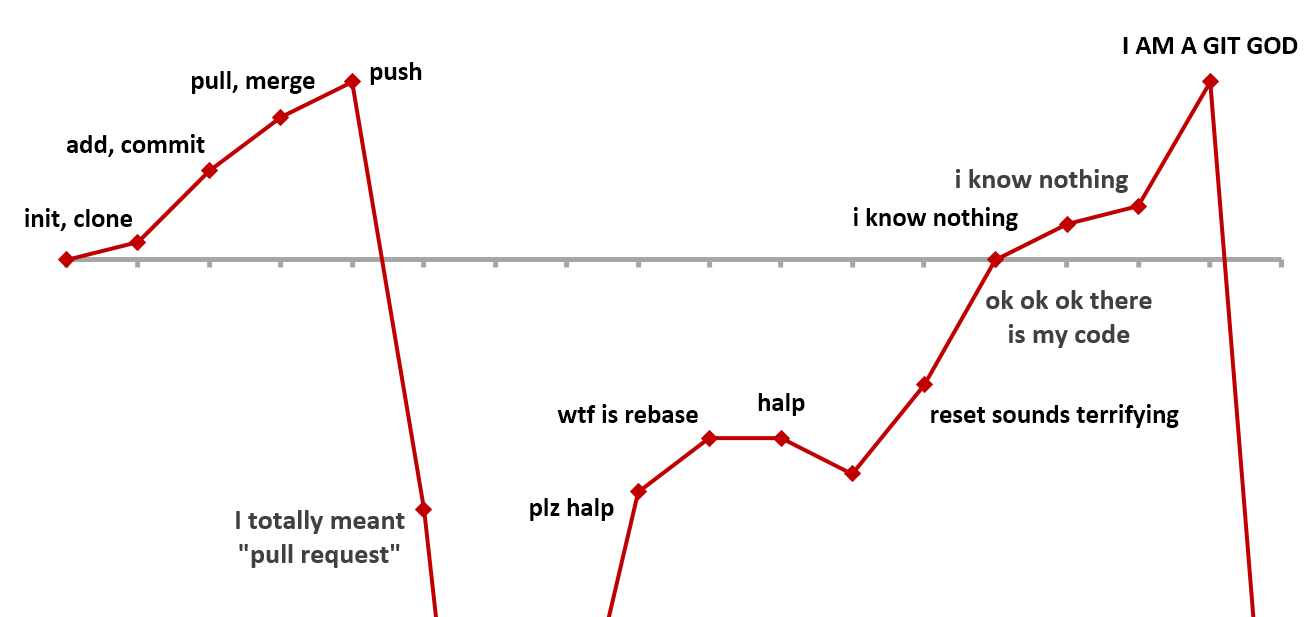
\includegraphics[width=0.75\textwidth]{Git-learning-curve}\\[2ex]
            \PB{\ldots{}but after all it is about having the correct mental set up!}
        \end{center}
        \begin{tikzpicture}[remember picture, overlay]
            \coordinate (center) at ($(figureStart)-(2.5mm,15mm)$);
            \draw[thick, PS, rotate around={30:(center)}] (center) ellipse (18mm and 8mm);
            \node[font=\small, text=PS, anchor=west] at ($(figureStart)+(14mm,-8mm)$) {This makes sense};
        \end{tikzpicture}
    \end{onlyenv}
    \begin{onlyenv}<2>
        \begin{itemize}
            \item As any new tool, it needs some practice
            \item \alert{The short- to long-term payoff is worth the effort}
            \item It is plenty of \URL[PP]{https://git-scm.com/downloads/guis/}{GUI clients}
                  \begin{itemize}
                      \item \URL[PB]{https://www.sourcetreeapp.com/}{Sourcetree:} A Free GIT Client For Windows And Mac
                      \item \URL[PB]{https://github.com/soramimi/Guitar}{Guitar:} Portable \Remark{Windows, Mac \& Linux}
                      \item \URL[PB]{https://git-cola.github.io/}{Git-Cola:} Powerful GUI For GIT \Remark{Windows, Mac, Ubuntu \& Linux}
                      \item{} [\ldots]
                  \end{itemize}
            \item You can work in the terminal\\ $\,\to\,$ after this course it will be possible and straightforward!
        \end{itemize}
    \end{onlyenv}
    \FrameRemark{Git was not designed to aim to user-friendliness, but it is by far the most used version control system in the world and hence in continuous evolution.}
\end{frame}
%~~~~~~~~~~~~~~~~~~~~~~~~~~~~~~~~~~~~~~~~~~~~%
\begin{frame}{Last but not least}
    \vspace{0.05\textheight}
    \begin{varblock}{}[0.95\textwidth]{Which large famous products are developed using Git?}
        Linux, Homebrew, Windows, Tensorflow, Angular, Inkscape, \ldots
    \end{varblock}
    \begin{varblock}{alert}[0.95\textwidth]{And if I do not have so large projects?}<2->
        It doesn't matter!
        There are too many advantages$^\star$ having a project under a source code management tool.
        Even alone.
        \textbf{Simply use one (Git).}
        \alert{\textbf{Now.}}
    \end{varblock}
    \vspace{-0.02\textheight}
    \begin{varblock}{alert}[0.95\textwidth]{}<2>
        \small
        For collaborative projects like maintaining code in a group, handing it over from person to person and so on, Git is simply a must.
        \textbf{As project leader, you should think about requiring everybody to work in a Git repository.}
    \end{varblock}
    \begin{tikzpicture}[remember picture, overlay]
        \node[anchor=north east, inner xsep=8mm, inner ysep=3mm] at (current page.north east) {
\includegraphics[width=0.25\textwidth]{Git-Logo}};
    \end{tikzpicture}
    \FrameRemark<2>{$^\star$ Among many others, in a Git repository you can undo a \texttt{rm} command given by accident on a wrong file.}
\end{frame}
%===============================================================%

%===============================================================%
\section{What is Git?}
%~~~~~~~~~~~~~~~~~~~~~~~~~~~~~~~~~~~~~~~~~~~~%
\begin{frame}{How does Git define itself?}
    \PrepareURLsymbol[PB]
    \begin{varblock}{quote}[0.95\textwidth]{}[\URL*{https://git-scm.com/}{Git homepage}]
        \guillemotleft
        Git is a free and open source distributed version control system designed to handle everything from small to very large projects with speed and efficiency.
        Git is easy to learn and has a tiny footprint with lightning fast performance.\guillemotright
        %It outclasses SCM tools like Subversion, CVS, Perforce, and ClearCase with features like cheap local branching, convenient staging areas, and multiple workflows.
    \end{varblock}
    \begin{enumerate}
        \item Free and open
        \item \textbf{Distributed version control system}
        \item \PP{From small to very large projects}
        \item With speed and efficiency
        \item \alert{Easy to learn}
    \end{enumerate}
\end{frame}
%~~~~~~~~~~~~~~~~~~~~~~~~~~~~~~~~~~~~~~~~~~~~%
\begin{frame}{How does it work?}
    \begin{overlayarea}{\textwidth}{0.75\textheight}
        \begin{itemize}
            \item \textbf{Repository:} a database containing all versions of the files
        \end{itemize}
        \begin{onlyenv}<1>
            \begin{center}
                \begin{tikzpicture}
                    \node (fig) {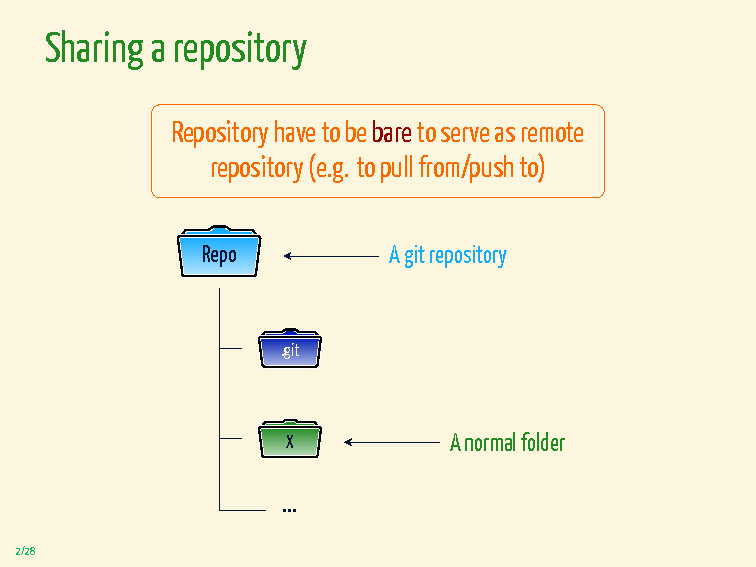
\includegraphics[width=0.8\textwidth, clip, trim=2cm 6mm 2cm 36mm]{Repository}};
                    \begin{DrawOnNode}{fig}
                        \fill[BGLIGHT] (0.3,0.9) rectangle (0.8,0.75);
                        \draw[from] (0.33,0.84) -- node[pos=1, right, text=PS] {Workspace} ++(0.285,0);
                        \draw[from] (0.44,0.56) -- node[pos=1, right, text=Navy, font=\small] {Local repository} ++(0.175,0);
                    \end{DrawOnNode}
                \end{tikzpicture}
            \end{center}
        \end{onlyenv}
        \begin{itemize}[<2->]
            \item Snapshot-based system
                  \begin{itemize}
                      \item Snapshots are called commits
                      \item Commits are named by checksums (also used to ensure data integrity)\\
                            \Remark{It's impossible to change the contents of any file or directory without Git knowing about it}
                  \end{itemize}
        \end{itemize}
        \begin{onlyenv}<2>
            \begin{center}
                  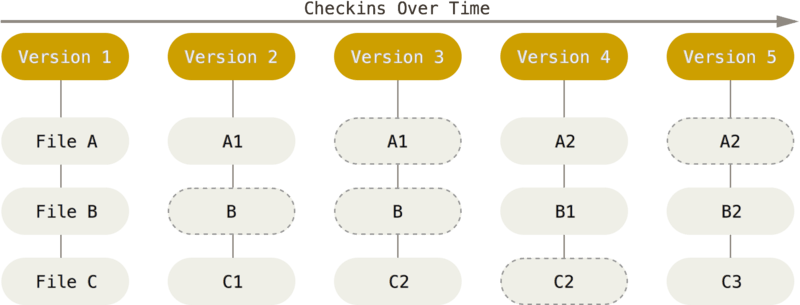
\includegraphics[width=0.75\textwidth]{Snapshots}\\
                  {\footnotesize\URL[PB]{https://git-scm.com/book/en/v2/Getting-Started-What-is-Git\%3F}{From the Git-Book}}
            \end{center}
        \end{onlyenv}
        \begin{itemize}[<3>]
            \item Almost every operation is local
                  \begin{itemize}
                      \item Working without network connecting
                      \item Distributed system $\,\to\,$ everyone carries a backup!
                  \end{itemize}
        \end{itemize}
        \PrepareURLsymbol[PB]
        \small
        \begin{varblock}{}[0.95\textwidth]{Are you curious to know how Git works bottom-up?}
            Refer to \URL*{http://ftp.newartisans.com/pub/git.from.bottom.up.pdf}{this 31-pages document}, well written, but not needed at start.
        \end{varblock}
    \end{overlayarea}
\end{frame}
%~~~~~~~~~~~~~~~~~~~~~~~~~~~~~~~~~~~~~~~~~~~~%
\begin{frame}{An example of Git history}
    \begin{center}
        \readlist\SHA{%
            6d7253af8a986838f78adc25a801cd06897be033
            54a94046deeb7117e77f0b6ee984165fedbc2345
            09c1b4321589b548be39063c828903901a3e14e7
            b924cdb3101220b552cdd92c8c4e7b9eb887a83a
            24ffea36e3b6b696cc537fbf05bae8d04c63a92b
        }
        \begin{varblock}{example}[0.9\textwidth]{}
            \small\PS{Every commit is a snapshot of the state of the repository at that point}
        \end{varblock}
        \begin{tikzpicture}
            \pgfmathsetmacro{\radius}{3mm}
            \pgfmathsetmacro{\dl}{2pt}
            \foreach \n[count=\i from 1] in {0,2,...,8}{
                \draw[line width=\dl pt, draw=PB, fill=PP!20] (\n,0) circle (\radius pt);
                \ifnum\i<5%
                    \draw (\n cm+\radius pt,0) -- ++(2 cm-2*\radius pt-0.5*\dl pt,0);
                \fi
                \node[rotate=90, font=\tiny, anchor=east] at (\n,-0.5) {\SHA[\i]};
            }
            \node[font=\small, text width=5ex, align=center, anchor=south, text=PB] at (0,0.5) {First commit};
            \node[font=\small, text width=3ex, align=center, anchor=south, text=PB] at (8,0.5) {HEAD};
        \end{tikzpicture}
    \end{center}
\end{frame}
%~~~~~~~~~~~~~~~~~~~~~~~~~~~~~~~~~~~~~~~~~~~~%
\begin{frame}{The correct abstract mental setup}
    \begin{uncoverenv}<2->
        \begin{tikzpicture}[node distance=5mm]
            \coordinate (N0) at (0,0);
            \foreach \n/\c [count=\i from 0, count=\ip from 1] in {Stashing area/PQ, Workspace/PS, Staging area/PP, Local repository/PB, Remote repository/PT}{
                \node[space=\c, right = of N\i] (N\ip) {\n};
                \draw[very thin] (N\ip) -- coordinate[pos=1] (E\ip) ++(0,-5);
            }
            \path coordinate (DNE) at ($(N4.north east)!0.5!(N5.north west)+(0,1)$)
                  coordinate (DSE) at ($(DNE)-(0,7.1)$)
                  coordinate (DNW) at ($(N1.north east)!0.5!(N2.north west)+(0,1)$)
                  coordinate (DSW) at ($(DNW)-(0,7.1)$);
            \draw[thin, dashed] (DNE) -- (DSE);
            \draw ($(N1.north west)-(0.1,0)$) -- ++(0,0.2) -| ($(N4.north east)+(0.1,0)$);
            \node[font=\small, anchor=south, inner sep=0pt] at ($(N1.north)!0.5!(N4.north)+(0,0.4)$) {Local machine};
            \node[draw=red, very thick, rounded corners=1mm, fill=yellow, text width=0.9\textwidth, align=center, font=\bfseries\large, text=red, visible on=<3>]
                at ($(N3.south)!0.5!(E3)$) {It's all about having this picture clear in mind and understand how git commands affect it};
            \begin{onlyenv}<4>
                \fill[Gray, fill opacity=0.95] (DNW) rectangle ($(DSW)-(2.3,0)$) node[pos=0.5, rotate=90, text=BGLIGHT, font=\large\bfseries] {Next part of the course};
                \fill[Gray, fill opacity=0.95] (DNE) rectangle ($(DSE)+(2.3,0)$) node[pos=0.5, rotate=90, text=BGLIGHT, font=\large\bfseries] {Next part of the course};
            \end{onlyenv}
        \end{tikzpicture}
    \end{uncoverenv}
\end{frame}
%===============================================================%

%===============================================================%
\section{How to use Git locally?}
%~~~~~~~~~~~~~~~~~~~~~~~~~~~~~~~~~~~~~~~~~~~~%
\begin{frame}[fragile]{Preliminary steps}{Be sure to introduce yourself to Git on \textbf{each} machine from which you work}
    \vspace{-0.02\textheight}
    \begin{enumerate}
        \item It is likely that Git is installed on your machine.
              \begin{itemize}
                  \item Check it in a terminal e.g.\ via \,\texttt{git version}
                  \item If needed, \URL[PB]{https://git-scm.com/book/en/v2/Getting-Started-Installing-Git}{install it}
              \end{itemize}
        \item Optionally, \URL[PB]{https://stackoverflow.com/a/18898614}{get/enable autocompletion in the terminal}
        \item Tell Git who you are and your email address\\
              {\small$\to\,$ this information will be used to sign your work in history}
    \end{enumerate}
    \begin{lstlisting}[style=MyBash, aboveskip=2mm]
        $ git config --global user.name 'Alessandro Sciarra'
        $ git config --global user.email 'sciarra@itp.uni-frankfurt.de'
    \end{lstlisting}
    \begin{enumerate}
        \setcounter{enumi}{3}
        \item Set your favourite editor e.g.\ to write commit messages
    \end{enumerate}
    \begin{lstlisting}[style=MyBash, aboveskip=2mm]
        $ git config --global core.editor 'emacs -nw'
    \end{lstlisting}
    \FrameRemark{The dollar symbol \,\texttt{\$}\, denotes the end of the prompt in the terminal. It will be from now on to denote commands to be used in the terminal.}
\end{frame}
%~~~~~~~~~~~~~~~~~~~~~~~~~~~~~~~~~~~~~~~~~~~~%
\begin{frame}{Asking for help about Git}
    \vspace{-0.05\textheight}
    \begin{enumerate}
        \item There are 3 ways in terminal\\[1mm]
              {\small
              \begin{tabular}{c@{\;}l@{\quad}c@{\quad}l}
                  \PP{$\circ$} & \texttt{git help <command>}   & e.g. & \texttt{git help config}   \\
                  \PP{$\circ$} & \texttt{git <command> --help} & e.g. & \texttt{git config --help} \\
                  \PP{$\circ$} & \texttt{man git-<command>}    & e.g. & \texttt{man git-config}    \\
              \end{tabular}}
        \item List of commands on the \URL[PB]{https://git-scm.com/docs}{official reference}
        \item Ask Google
    \end{enumerate}
    \medskip
    \PrepareURLsymbol[PQ]
    \begin{varblock}{alert}[0.9\textwidth]{There is plenty of cheat-sheets online:}
        \URL*{https://education.github.com/git-cheat-sheet-education.pdf}{GitHub education}
        \qquad
        \URL*{https://about.gitlab.com/images/press/git-cheat-sheet.pdf}{GitLab}
        \qquad
        \URL*{https://www.atlassian.com/git/tutorials/atlassian-git-cheatsheet}{Bitbucket}
    \end{varblock}
    \FrameRemark{Every \;\texttt{git <command>}\; can be referred to as \;\texttt{git-command}, although the first notation has to be used to run the command.}
\end{frame}
%~~~~~~~~~~~~~~~~~~~~~~~~~~~~~~~~~~~~~~~~~~~~%
\begin{frame}[fragile]{Creating a repository}{It is as simple as running one command}
    \begin{lstlisting}[style=MyBash]
        $ git config --get user.name
        Alessandro Sciarra
        $ git config --get user.email
        sciarra@itp.uni-frankfurt.de
        # Suppose to be in a folder you want to turn into a repository
        $ pwd
        |+/home/asciarra/Documents/first-repo+|
        $ ls -a
        @|\ttc{Blue}{.~~..}~~Paper.aux~~Paper.log~~Paper.out~~Paper.pdf~~Paper.tex|@
    \end{lstlisting}
    \begin{uncoverenv}<2->
        \begin{lstlisting}[style=MyBash]
            $ git init  # <--- Here you go!
            |+Initialised empty Git repository in ~/Documents/first-repo/.git/+|
            $ ls -a
            @|\ttc{Blue}{.~~..~~.git}~~Paper.aux~~Paper.log~~Paper.out~~Paper.pdf~~Paper.tex|@
        \end{lstlisting}
    \end{uncoverenv}
    \begin{varblock}{alert}[0.9\textwidth]{Do not shoot yourself!}<3>
        \PQ{Never ever touch by hand the content of the \,\texttt{.git}\, folder.}
    \end{varblock}
\end{frame}
%~~~~~~~~~~~~~~~~~~~~~~~~~~~~~~~~~~~~~~~~~~~~%
\newcommand{\GitCommand}[6][midway]{%
    \draw[#2] ($(N#3.south)!#5!(E#3)$) -- node[#1, fill=BGLIGHT, font=\ttfamily\scriptsize] {#6} ($(N#4.south)!#5!(E#4)$);
}
\begin{frame}<1-3>[label=gitLocal]{\alt<1-3>{What comes next?}{Back to our mental picture}}{\only<2->{On your local machine}}
    \vspace{-0.1\textheight}
    \begin{center}
        \begin{tikzpicture}[node distance=25mm]
            \begin{scope}[scope on=<2->]
                \coordinate (N0) at (0,0);
                \foreach \n/\c [count=\i from 0, count=\ip from 1] in {Workspace/PS, Staging area/PP, Local repository/PB}{
                    \node[space=\c, right = of N\i] (N\ip) {\n};
                    \draw[very thin] (N\ip) -- coordinate[pos=1] (E\ip) ++(0,-5);
                }
            \end{scope}
            \begin{scope}[scope on=<3->]
                \node[text=PQ, font=\ttfamily\scriptsize] at ($(N1)!0.5!(N2)$) {git status};
                \node[text=PQ, font=\ttfamily\scriptsize] at ($(N3.north)+(0,0.3)$) {git log};
                \node[text=PQ, font=\ttfamily\scriptsize] at ($(N3.north)+(0,0.7)$) {git show};
                \GitCommand{fromto,PQ}{1}{2}{0.10}{git diff}
                \GitCommand{fromto,PQ}{2}{3}{0.25}{git diff --staged}
                \GitCommand{to}{1}{2}{0.65}{git add}
                \GitCommand{from}{1}{2}{0.80}{git restore --staged}
                \GitCommand{to}{2}{3}{0.95}{git commit}
                \path[to, PQ] ($($(N3.south)!0.45!(E3)$)!0.65!($(N2.south)!0.45!(E2)$)$) edge[out=180, in=0] ($(N2.south)!0.35!(E2)$);
                \GitCommand[pos=0.8]{fromto,PQ}{1}{3}{0.45}{git diff HEAD}
                \node[text=PT] at ($($(N1.south)!0.47!(E1)$)!0.8!($(N3.south)!0.51!(E3)$)$) {\Remark{only tracked files}};
            \end{scope}
        \end{tikzpicture}
        \par\medskip
        \uncover<2->{\small Commands marked in \PQ{dark red} do not change anything in the repository!}
        \FrameRemark<3->{Git introduced \;\texttt{git\,restore}\; in v2.23 but this stayed buggy for a while. Use it from v2.27 on, otherwhise use \;\texttt{git\,reset}.}
    \end{center}
\end{frame}
%~~~~~~~~~~~~~~~~~~~~~~~~~~~~~~~~~~~~~~~~~~~~%
\begin{frame}[fragile]{Git status}
    \begin{lstlisting}[style=MyBash]
        $ git status
        |+On branch main+|

        |+No commits yet+|

        |+Untracked files:+|
        |+  (use "git add <file>..." to include in what will be committed)+|
        @|\ttc{red}{~~~~~Paper.aux}|@
        @|\ttc{red}{~~~~~Paper.log}|@
        @|\ttc{red}{~~~~~Paper.out}|@
        @|\ttc{red}{~~~~~Paper.pdf}|@
        @|\ttc{red}{~~~~~Paper.tex}|@

        |+nothing added to commit but untracked files present+|
        |+(use "git add" to track)+|
    \end{lstlisting}
    \begin{varblock}{alert}[0.95\textwidth]{You do not want to put everything in a repository!}
        It is possible to tell git to ignore some files, like temporary ones
    \end{varblock}
\end{frame}
%~~~~~~~~~~~~~~~~~~~~~~~~~~~~~~~~~~~~~~~~~~~~%
\begin{frame}[fragile]{Letting Git ignore some files}
    \begin{lstlisting}[style=MyBash]
        $ printf '*.%s\n' aux log out pdf > .gitignore
        $ cat .gitignore
        |+*.aux+|
        |+*.log+|
        |+*.out+|
        |+*.pdf+|
        $ git status
        |+On branch main+|

        |+No commits yet+|

        |+Untracked files:+|
        |+  (use "git add <file>..." to include in what will be committed)+|
        @|\ttc{red}{~~~~~.gitignore}|@
        @|\ttc{red}{~~~~~Paper.tex}|@

        |+nothing added to commit but untracked files present+|
        |+(use "git add" to track)+|
    \end{lstlisting}
    \begin{center}
        \URL[PB]{https://github.com/github/gitignore}{github/gitignore}
        \qquad
        \URL[PP]{https://github.com/github/gitignore/blob/main/TeX.gitignore}{for LaTeX projects}
    \end{center}
\end{frame}
%~~~~~~~~~~~~~~~~~~~~~~~~~~~~~~~~~~~~~~~~~~~~%
\begin{frame}[fragile]{Our first commit}
    \vspace{-0.09\textheight}
    \begin{overlayarea}{\textwidth}{0.7\textheight}
        \begin{onlyenv}<1>
            \centerline{In your terminal}
            \begin{lstlisting}[style=MyBash, aboveskip=2mm, xleftmargin=-1mm, xrightmargin=-1mm]
                $ git log
                |+fatal: your current branch 'main' does not have any commits yet+|
                $ git add .gitignore
                $ git status
                |+On branch main+|

                |+No commits yet+|

                |+Changes to be committed:+|
                |+  (use "git rm --cached <file>..." to unstage)+|
                @|\ttc{ForestGreen}{~~~~~new file:~~~.gitignore}|@

                |+Untracked files:+|
                |+  (use "git add <file>..." to include in what will be committed)+|
                @|\ttc{red}{~~~~~Paper.tex}|@
                $ git commit
            \end{lstlisting}
        \end{onlyenv}
        \begin{onlyenv}<2>
            \centerline{In your favourite editor}
            \begin{lstlisting}[style=MyBash, aboveskip=2mm, xleftmargin=-3mm, xrightmargin=-3mm]
                @|\raisebox{-0.5pt}{\tikz[] \fill[black] (0,0) rectangle (0.13,0.23);}|@

                # Please enter the commit message for your changes. Lines starting
                # with '#' will be ignored, and an empty message aborts the commit.
                #
                # On branch @|\ttc{DarkOrange}{main}|@
                #
                # Initial commit
                #
                # @|\ttc{Goldenrod}{Changes to be committed:}|@
                #       new file:   @|\ttc{ForestGreen}{.gitignore}|@
                #
                # @|\ttc{Goldenrod}{Untracked files:}|@
                #       @|\ttc{ForestGreen}{Paper.tex}|@
                #
            \end{lstlisting}
        \end{onlyenv}
        \begin{onlyenv}<3>
            \centerline{In your favourite editor}
            \begin{lstlisting}[style=MyBash, aboveskip=2mm, xleftmargin=-3mm, xrightmargin=-3mm]
                |+Add .gitignore file for TeX project+|@|\,\raisebox{-0.5pt}{\tikz \fill[black] (0,0) rectangle (0.13,0.23);}|@

                # Please enter the commit message for your changes. Lines starting
                # with '#' will be ignored, and an empty message aborts the commit.
                #
                # On branch @|\ttc{DarkOrange}{main}|@
                #
                # Initial commit
                #
                # @|\ttc{Goldenrod}{Changes to be committed:}|@
                #       new file:   @|\ttc{ForestGreen}{.gitignore}|@
                #
                # @|\ttc{Goldenrod}{Untracked files:}|@
                #       @|\ttc{ForestGreen}{Paper.tex}|@
                #
            \end{lstlisting}
        \end{onlyenv}
        \begin{onlyenv}<4>
            \centerline{In your terminal}
            \begin{lstlisting}[style=MyBash, aboveskip=2mm, xleftmargin=-2mm, xrightmargin=-2mm]
                $ git log
                |+fatal: your current branch 'main' does not have any commits yet+|
                $ git add .gitignore
                $ git status
                |+On branch main+|

                |+No commits yet+|

                |+Changes to be committed:+|
                |+  (use "git rm --cached <file>..." to unstage)+|
                @|\ttfamily\color{ForestGreen}~~~~~new file:~~~.gitignore|@

                |+Untracked files:+|
                |+  (use "git add <file>..." to include in what will be committed)+|
                @|\ttfamily\color{red}~~~~~Paper.tex|@
                $ git commit
                # Your editor opens -> type commit message, save and exit
                |+[main (root-commit) bb8c78b] Add .gitignore file for TeX project+|
                |+ 1 file changed, 4 insertions(+)+|
                |+ create mode 100644 .gitignore+|
            \end{lstlisting}
        \end{onlyenv}
    \end{overlayarea}
\end{frame}
%~~~~~~~~~~~~~~~~~~~~~~~~~~~~~~~~~~~~~~~~~~~~%
\begin{frame}[fragile]{Inspecting history}
    \begin{lstlisting}[style=MyBash, belowskip=-4mm]
        $ git log
        |+commit bb8c78b68075dacf8467420bc00867c73ef5ba8c (HEAD -> main)+|
        |+Author: Alessandro Sciarra <asciarra@fias.uni-frankfurt.de>+|
        |+Date:   Thu Dec 23 10:13:05 2021 +0100+|

        |+    Add .gitignore file for TeX project+|
        $ git log --oneline
        |+bb8c78b (HEAD -> main) Add .gitignore file for LaTeX project+|
    \end{lstlisting}
    \centerline{Use a pager to avoid polluting terminal}
    \begin{lstlisting}[style=MyBash, aboveskip=2mm]
        $ git config --global core.pager 'less -+$LESS -R'
    \end{lstlisting}
    \medskip
    \begin{varblock}{}[0.8\textwidth]{}
        Use \;\PB{\texttt{git show}}\; or \;\PB{\texttt{git show <SHA1>}}\; to inspect what has been done in last or given commit
    \end{varblock}
\end{frame}
%~~~~~~~~~~~~~~~~~~~~~~~~~~~~~~~~~~~~~~~~~~~~%
\begin{frame}[fragile]{Our second commit}
    \begin{lstlisting}[style=MyBash]
        $ git status
        |+On branch main+|
        |+Untracked files:+|
        |+  (use "git add <file>..." to include in what will be committed)+|
            @|\ttc{red}{Paper.tex}|@

        |+nothing added to commit but untracked files present+|
        |+(use "git add" to track)+|
        $ git add Paper.tex # Always add to the staging
                            # area before committing!
        $ git status
        |+On branch main+|
        |+Changes to be committed:+|
        |+  (use "git restore --staged <file>..." to unstage)+|
               @|\ttc{ForestGreen}{new file:   Paper.tex}|@
        $ git commit -m 'Add paper main document'
        |+[main 9c6154d] Add paper main document+|
        |+ 1 file changed, 147 insertions(+)+|
        |+ create mode 100644 Paper.tex+|
    \end{lstlisting}
\end{frame}
%~~~~~~~~~~~~~~~~~~~~~~~~~~~~~~~~~~~~~~~~~~~~%
\begin{frame}[fragile]{Use good commit messages}
    \begin{lstlisting}[style=MyBash]
        $ git log --oneline
        |+9c6154d (HEAD -> main) Add paper main document+|
        |+bb8c78b Add .gitignore file for LaTeX project+|
    \end{lstlisting}
    \vspace{1mm}
    \begin{itemize}
        \item Write them like an email to yourself (or to the other developers)\\
              $\to\;$ Subject line + body, follow \URL[PB]{https://p5v.medium.com/what-s-with-the-50-72-rule-8a906f61f09c}{the 50/72 rule}
        \item Subject: Summarize what has been done\\
              $\to\;$ \alert{\textbf{Use present tense and no period at the end!}}
        \item Body: \PP{After empty line}, document why you made the changes\\[-0.5ex]
              \phantom{Bo}$\drsh$\Remark{add one only if needed}
    \end{itemize}
    \begin{varblock}{alert}[0.98\textwidth]{Good commits}
        Commit small and conceptually separated changes, commit often and do not add binary files to your repository.
    \end{varblock}
    \FrameRemark{In coding projects, although not always possible/trivial, try to commit working/compiling code.}
\end{frame}
%~~~~~~~~~~~~~~~~~~~~~~~~~~~~~~~~~~~~~~~~~~~~%
\againframe<4>[noframenumbering, plain]{gitLocal}
%~~~~~~~~~~~~~~~~~~~~~~~~~~~~~~~~~~~~~~~~~~~~%
\begin{frame}[fragile]{Working and displaying changes}
    \vspace{-0.0\textheight}
    \begin{overlayarea}{\textwidth}{0.7\textheight}
        \begin{onlyenv}<1>
            \centerline{In your terminal}
            \begin{lstlisting}[style=MyBash, aboveskip=2mm, xleftmargin=-6mm, xrightmargin=-6mm]
                # Make some changes
                $ git status
                |+On branch main+|
                |+Changes not staged for commit:+|
                |+  (use "git add <file>..." to update what will be committed)+|
                |+  (use "git restore <file>..." to discard changes in working directory)+|
                    @|\ttc{red}{modified:   Paper.tex}|@

                |+no changes added to commit (use "git add" and/or "git commit -a")+|
                $ git diff
            \end{lstlisting}
        \end{onlyenv}
        \begin{onlyenv}<2>
            \centerline{In your pager, e.g.\ \bash|less|}
            \begin{lstlisting}[style=MyBash, aboveskip=2mm]
                |+diff --git a/Paper.tex b/Paper.tex+|
                |+index 3c408e5..3669114 100644+|
                |+--- a/Paper.tex+|
                |++++ b/Paper.tex+|
                @|\ttc{DarkTurquoise}{@@ -42,7 +42,7 @@}|@ |+pdftitle={LaTeX Seminar for PhD students}+|
                |+     {Sprecher \& Seminarleiter}%+|
                |+ }+|

                @|\ttc{red}{-\textbackslash date\{\textbackslash \today\}}|@
                @|\ttc{ForestGreen}{+\textbackslash date\{23. Dezember 2021\}}|@

                |+ \newcommand{\etc}{etc.}+|
                |+ \newcommand{\zB}{z.B.}+|
            \end{lstlisting}
        \end{onlyenv}
        \begin{onlyenv}<3>
            \centerline{In your terminal}
            \begin{lstlisting}[style=MyBash, aboveskip=2mm, xleftmargin=-6mm, xrightmargin=-6mm]
                # Make some changes
                $ git status
                |+On branch main+|
                |+Changes not staged for commit:+|
                |+  (use "git add <file>..." to update what will be committed)+|
                |+  (use "git restore <file>..." to discard changes in working directory)+|
                    @|\ttc{red}{modified:   Paper.tex}|@

                |+no changes added to commit (use "git add" and/or "git commit -a")+|
                $ git diff
                $ git diff --staged  # Nothing in the staging area!
                $ git add Paper.tex
                $ git diff           # No changes anymore in the workspace!
                $ git diff --staged  # Our changes are now staged
                $ git commit -m 'Fix date for main document'
                # ...
            \end{lstlisting}
        \end{onlyenv}
    \end{overlayarea}
\end{frame}
%~~~~~~~~~~~~~~~~~~~~~~~~~~~~~~~~~~~~~~~~~~~~%
\begin{frame}[fragile]{What else can I easily explore?}
    \begin{itemize}
        \item Stage all tracked modified files at once\\[1mm]
              \begin{minipage}{\linewidth}
                  \begin{lstlisting}[style=MyBash]
                      git add -u
                  \end{lstlisting}
              \end{minipage}
        \item Stage partial modification in a file\\[1mm]
              \begin{minipage}{\linewidth}
                  \begin{lstlisting}[style=MyBash]
                      git add -p
                  \end{lstlisting}
              \end{minipage}
        \item Define your aliases\\[1mm]
              \begin{minipage}{\linewidth}
                  \begin{lstlisting}[style=MyBash]
                      git config --global alias.unstage 'restore --staged --'
                      # From now on, you can use 'git unstage'
                  \end{lstlisting}
              \end{minipage}
        \item Let git correct you when you mistype$^\star$\\[1mm]
              \begin{minipage}{\linewidth}
                  \begin{lstlisting}[style=MyBash]
                      git config --global help.autocorrect 1
                  \end{lstlisting}
              \end{minipage}
        \item Change/correct your last commit message
              \begin{minipage}{\linewidth}
                  \begin{lstlisting}[style=MyBash]
                      git commit --amend
                  \end{lstlisting}
              \end{minipage}
    \end{itemize}
    \FrameRemark{$^\star$ If you want a friend to correct your mistyped last command \textbf{in general} in the terminal, check-out \URL*{https://github.com/nvbn/thefuck}{this hilarious project}.}
\end{frame}
%===============================================================%

%===============================================================%
\section{Summary and conclusions}
%~~~~~~~~~~~~~~~~~~~~~~~~~~~~~~~~~~~~~~~~~~~~%
\begin{frame}{Your workflow from now on, right?}
    \begin{center}
        \begin{tikzpicture}[node distance=3mm, bezier bounding box] % \usetikzlibrary{bbox}
            \coordinate (N0) at (0,0);
            \foreach \n/\c [count=\i from 0, count=\ip from 1] in {Work/PS, git status git diff/PP, git add/PB, git commit/PT}{
                \begin{scope}[scope on=<\ip->]
                    \node[space=\c, below = of N\i, xshift=25mm] (N\ip) {\n};
                    \ifnum\i>0%
                        \path[thick, to] (N\i.east) edge[out=0, in=90] (N\ip.north);
                    \fi
                \end{scope}
            }
            \path[visible on=<5->, thick, dotted, to] (N4.west) edge[out=180, in=180, looseness=1.6] (N2.west);
            \path[visible on=<6->, thick, to] (N4.south) edge[out=270, in=180, looseness=1.3] (N1.west);
        \end{tikzpicture}
    \end{center}
\end{frame}
%~~~~~~~~~~~~~~~~~~~~~~~~~~~~~~~~~~~~~~~~~~~~%
\begin{frame}{That's \textbf{NOT} all folks}
    \vspace{0.02\textheight}
    \begin{enumerate}[<+->]
        \item Start using Git.
              \alert{\textbf{Now.}}
              Not tomorrow or next week, today!\\
              $\to\;$ Repeat what done on these slides
        \item Was anything unclear?
              Did you get stuck at some point?\\
              $\to\;$ Drop me \PP{\href{mailto:sciarra@itp.uni-frankfurt.de}{{\small\faEnvelope}\;an email}}
        \item Git is much more than this!\\
              $\to\;$ Attend next part: \alert{\guillemotleft Let's git \textbf{together}\tikzmark{tg}\guillemotright}
    \end{enumerate}
    \begin{tikzpicture}[remember picture, overlay, scope on=<.->]
        \node[anchor=west, space=PT, text width=18mm] (content) at ($(tg)+(0.5,-0.8)$) {
            git clone\\
            git branch\\
            git switch\\
            git checkout\\
            git merge\\
            git pull\\
            git push
        };
        \path[to, shorter={0mm}{1mm}] ($(tg)-(0.6,0.25)$) edge[out=270, in=180] (content.west);
    \end{tikzpicture}
    \par\vspace{0.02\textheight}
    \begin{uncoverenv}<+->
        \begin{tikzpicture}[remember picture, overlay]
            \node[anchor=north east, cloud, aspect=3, cloud puffs=15, draw=PB, fill=PP!20, text=PB]
                at ($(current page.north east)+(-14mm,-6mm)$) {Thank you!};
        \end{tikzpicture}
        \begin{minipage}{0.8\textwidth}
            \begin{center}
                \large\bfseries\PQ{Believe me, it's worth it!}
            \end{center}
        \end{minipage}
    \end{uncoverenv}
\end{frame}
%===============================================================%

\end{document}
